%% For double-blind review submission, w/o CCS and ACM Reference (max submission space)
% \documentclass[sigplan,review,anonymous]{acmart}\settopmatter{printfolios=true,printccs=false,printacmref=false}
% \documentclass[sigplan,10pt,review,anonymous]{acmart}\settopmatter{printfolios=true,printccs=false,printacmref=false} 
\documentclass[sigplan,10pt,review]{acmart}\settopmatter{printfolios=true,printccs=false,printacmref=false} 
%% For double-blind review submission, w/ CCS and ACM Reference
%\documentclass[sigplan,review,anonymous]{acmart}\settopmatter{printfolios=true}
%% For single-blind review submission, w/o CCS and ACM Reference (max submission space)
%\documentclass[sigplan,review]{acmart}\settopmatter{printfolios=true,printccs=false,printacmref=false}
%% For single-blind review submission, w/ CCS and ACM Reference
%\documentclass[sigplan,review]{acmart}\settopmatter{printfolios=true}
%% For final camera-ready submission, w/ required CCS and ACM Reference
%\documentclass[sigplan]{acmart}\settopmatter{}


%% Conference information
%% Supplied to authors by publisher for camera-ready submission;
%% use defaults for review submission.
\acmConference[PL'18]{ACM SIGPLAN Conference on Programming Languages}{January 01--03, 2018}{New York, NY, USA}
\acmYear{2018}
\acmISBN{} % \acmISBN{978-x-xxxx-xxxx-x/YY/MM}
\acmDOI{} % \acmDOI{10.1145/nnnnnnn.nnnnnnn}
\startPage{1}

%% Copyright information
%% Supplied to authors (based on authors' rights management selection;
%% see authors.acm.org) by publisher for camera-ready submission;
%% use 'none' for review submission.
\setcopyright{none}
%\setcopyright{acmcopyright}
%\setcopyright{acmlicensed}
%\setcopyright{rightsretained}
%\copyrightyear{2018}           %% If different from \acmYear

%% Bibliography style
\bibliographystyle{ACM-Reference-Format}
%% Citation style
%\citestyle{acmauthoryear}  %% For author/year citations
%\citestyle{acmnumeric}     %% For numeric citations
%\setcitestyle{nosort}      %% With 'acmnumeric', to disable automatic
                            %% sorting of references within a single citation;
                            %% e.g., \cite{Smith99,Carpenter05,Baker12}
                            %% rendered as [14,5,2] rather than [2,5,14].
%\setcitesyle{nocompress}   %% With 'acmnumeric', to disable automatic
                            %% compression of sequential references within a
                            %% single citation;
                            %% e.g., \cite{Baker12,Baker14,Baker16}
                            %% rendered as [2,3,4] rather than [2-4].


%%%%%%%%%%%%%%%%%%%%%%%%%%%%%%%%%%%%%%%%%%%%%%%%%%%%%%%%%%%%%%%%%%%%%%
%% Note: Authors migrating a paper from traditional SIGPLAN
%% proceedings format to PACMPL format must update the
%% '\documentclass' and topmatter commands above; see
%% 'acmart-pacmpl-template.tex'.
%%%%%%%%%%%%%%%%%%%%%%%%%%%%%%%%%%%%%%%%%%%%%%%%%%%%%%%%%%%%%%%%%%%%%%


%% Some recommended packages.
\usepackage{booktabs}   %% For formal tables:
                        %% http://ctan.org/pkg/booktabs
\usepackage{subcaption} %% For complex figures with subfigures/subcaptions
                        %% http://ctan.org/pkg/subcaption

% Packages usually used by soton
	% Package for input encoding
	\usepackage[utf8]{inputenc}
	
	%\usepackage[T1]{fontenc}
	%\usepackage{lmodern}
	
	% Package for multilingual support, loaded with English support.
	\usepackage[english]{babel}
	
	% Package for fancy quotations
	\usepackage[autostyle]{csquotes}
	
	% Package for URLs
	\usepackage{url}
	
%	\usepackage{colourSoton}
	
	% Package for hyper-references
	\usepackage{hyperref}
	\hypersetup{
		colorlinks=true,
		citecolor=red,
		linkcolor=blue,
		urlcolor=cyan,
	}
	
	% Package for graphics
	\usepackage{graphicx}
	\graphicspath{ {img/} }
	
	% Package for change tracking
	% \usepackage{chgtrk}
	% \newCTcontributor{Tomas}
	% \newCTcontributor{Colin}
	% \newCTcontributor{Son}
	% \newCTcontributor{Dana}
	% \newCTcontributor{Rupert}
	% \newCTcontributor{Keming}
	% \newCTcontributor{Michael}
	
	% Package for abbreviation
	\usepackage{abbrev-scxml2020}
	
	% Package for standalone source code
	\usepackage{standalone}
	
	% Package for requirements document
%	\usepackage[compact]{reqdoc}
	
	% Package for TikZ pictures
	\usepackage{tikz}
	\usetikzlibrary{positioning}
	\usetikzlibrary{shapes}
	
	% Custom pgf pictures
%	\usepackage{pgf-picture}
	
	\usepackage{wrapfig}
	
	% Package for listing Event-B code
	\usepackage[colour]{lstEventB}
	
	% Package for listing Gherkin code
%	\usepackage[colour]{lstGherkin}
	
	%package for envelope
	\usepackage{bbding}
% end of packages used by soton

\begin{document}

%% Title information
% \title[Short Title]{Full Title}         %% [Short Title] is optional;
\title[]{Refinement of Reactive Systems}         %% [Short Title] is optional;
                                        %% when present, will be used in
                                        %% header instead of Full Title.
\titlenote{with title note}             %% \titlenote is optional;
                                        %% can be repeated if necessary;
                                        %% contents suppressed with 'anonymous'
\subtitle{Subtitle}                     %% \subtitle is optional
\subtitlenote{with subtitle note}       %% \subtitlenote is optional;
                                        %% can be repeated if necessary;
                                        %% contents suppressed with 'anonymous'


%% Author information
%% Contents and number of authors suppressed with 'anonymous'.
%% Each author should be introduced by \author, followed by
%% \authornote (optional), \orcid (optional), \affiliation, and
%% \email.
%% An author may have multiple affiliations and/or emails; repeat the
%% appropriate command.
%% Many elements are not rendered, but should be provided for metadata
%% extraction tools.

%% Author with single affiliation.
\author{First1 Last1}
\authornote{with author1 note}          %% \authornote is optional;
                                        %% can be repeated if necessary
\orcid{nnnn-nnnn-nnnn-nnnn}             %% \orcid is optional
\affiliation{
  \position{Position1}
  \department{Department1}              %% \department is recommended
  \institution{Institution1}            %% \institution is required
  \streetaddress{Street1 Address1}
  \city{City1}
  \state{State1}
  \postcode{Post-Code1}
  \country{Country1}                    %% \country is recommended
}
\email{first1.last1@inst1.edu}          %% \email is recommended

%% Author with two affiliations and emails.
\author{First2 Last2}
\authornote{with author2 note}          %% \authornote is optional;
                                        %% can be repeated if necessary
\orcid{nnnn-nnnn-nnnn-nnnn}             %% \orcid is optional
\affiliation{
  \position{Position2a}
  \department{Department2a}             %% \department is recommended
  \institution{Institution2a}           %% \institution is required
  \streetaddress{Street2a Address2a}
  \city{City2a}
  \state{State2a}
  \postcode{Post-Code2a}
  \country{Country2a}                   %% \country is recommended
}
\email{first2.last2@inst2a.com}         %% \email is recommended
\affiliation{
  \position{Position2b}
  \department{Department2b}             %% \department is recommended
  \institution{Institution2b}           %% \institution is required
  \streetaddress{Street3b Address2b}
  \city{City2b}
  \state{State2b}
  \postcode{Post-Code2b}
  \country{Country2b}                   %% \country is recommended
}
\email{first2.last2@inst2b.org}         %% \email is recommended


%% Abstract
%% Note: \begin{abstract}...\end{abstract} environment must come
%% before \maketitle command
% \begin{abstract}
% Text of abstract \ldots.
% \end{abstract}
% !TEX root = ../main.tex
\begin{abstract}
Text of abstract 
\end{abstract}

%% 2012 ACM Computing Classification System (CSS) concepts
%% Generate at 'http://dl.acm.org/ccs/ccs.cfm'.
\begin{CCSXML}
<ccs2012>
<concept>
<concept_id>10011007.10011006.10011008</concept_id>
<concept_desc>Software and its engineering~General programming languages</concept_desc>
<concept_significance>500</concept_significance>
</concept>
<concept>
<concept_id>10003456.10003457.10003521.10003525</concept_id>
<concept_desc>Social and professional topics~History of programming languages</concept_desc>
<concept_significance>300</concept_significance>
</concept>
</ccs2012>
\end{CCSXML}

\ccsdesc[500]{Software and its engineering~General programming languages}
\ccsdesc[300]{Social and professional topics~History of programming languages}
%% End of generated code


%% Keywords
%% comma separated list
% \keywords{keyword1, keyword2, keyword3}  %% \keywords are mandatory in final camera-ready submission
\keywords{run-to-completion, refinement}  %% \keywords are mandatory in final camera-ready submission


%% \maketitle
%% Note: \maketitle command must come after title commands, author
%% commands, abstract environment, Computing Classification System
%% environment and commands, and keywords command.
\maketitle


\section{Introduction}
We formalise the semantics of refinement in SCXML by modelling, in Event-B,
\begin{itemize}
	\item the structure and behaviour of abstract SCXML models,
	\item the structure, behaviour of refined SCXML models and their relationship to abstract models.
	\item We then refine the latter to remove verification artifacts and show that it is no different to the abstract model and hence SCXML refinement can be applied iteratively.
\end{itemize}

Since SCXML consists of a state-chart behaviour superimposed with a 'run to completion' execution semantics, we formalise the refinement of these two parts separately and then compose the two definitions to obtain the complete SCXMl refinement semantics.
% \section{Introduction}
% Text of paper \ldots
% !TEX root = ../main.tex


\section{Background and Previous Work}
% !TEX root = ../main.tex


\section{Run To Completion}
\label{sec:run-completion}
The run to completion semantics is specified via an abstract basis that is extended by the model~\cite{MoSnHo18,MoSnHo-ABZ2020}. 
Figure~\ref{fig:basis} shows a state-chart representation of how the basis enforces 
the run to completion semantics on the model transitions. 

\ColinInlineComment{the Fig.1 needs updating wrt to queues.. e.g. eQ and iQ should be content(eQ) and content(iQ).
	also NoTriggeredTransitionsEnable should be NoTriggeredTransitionsEnabled}
\begin{figure}[!h]
	\vspace{-.4cm}
	\centering
	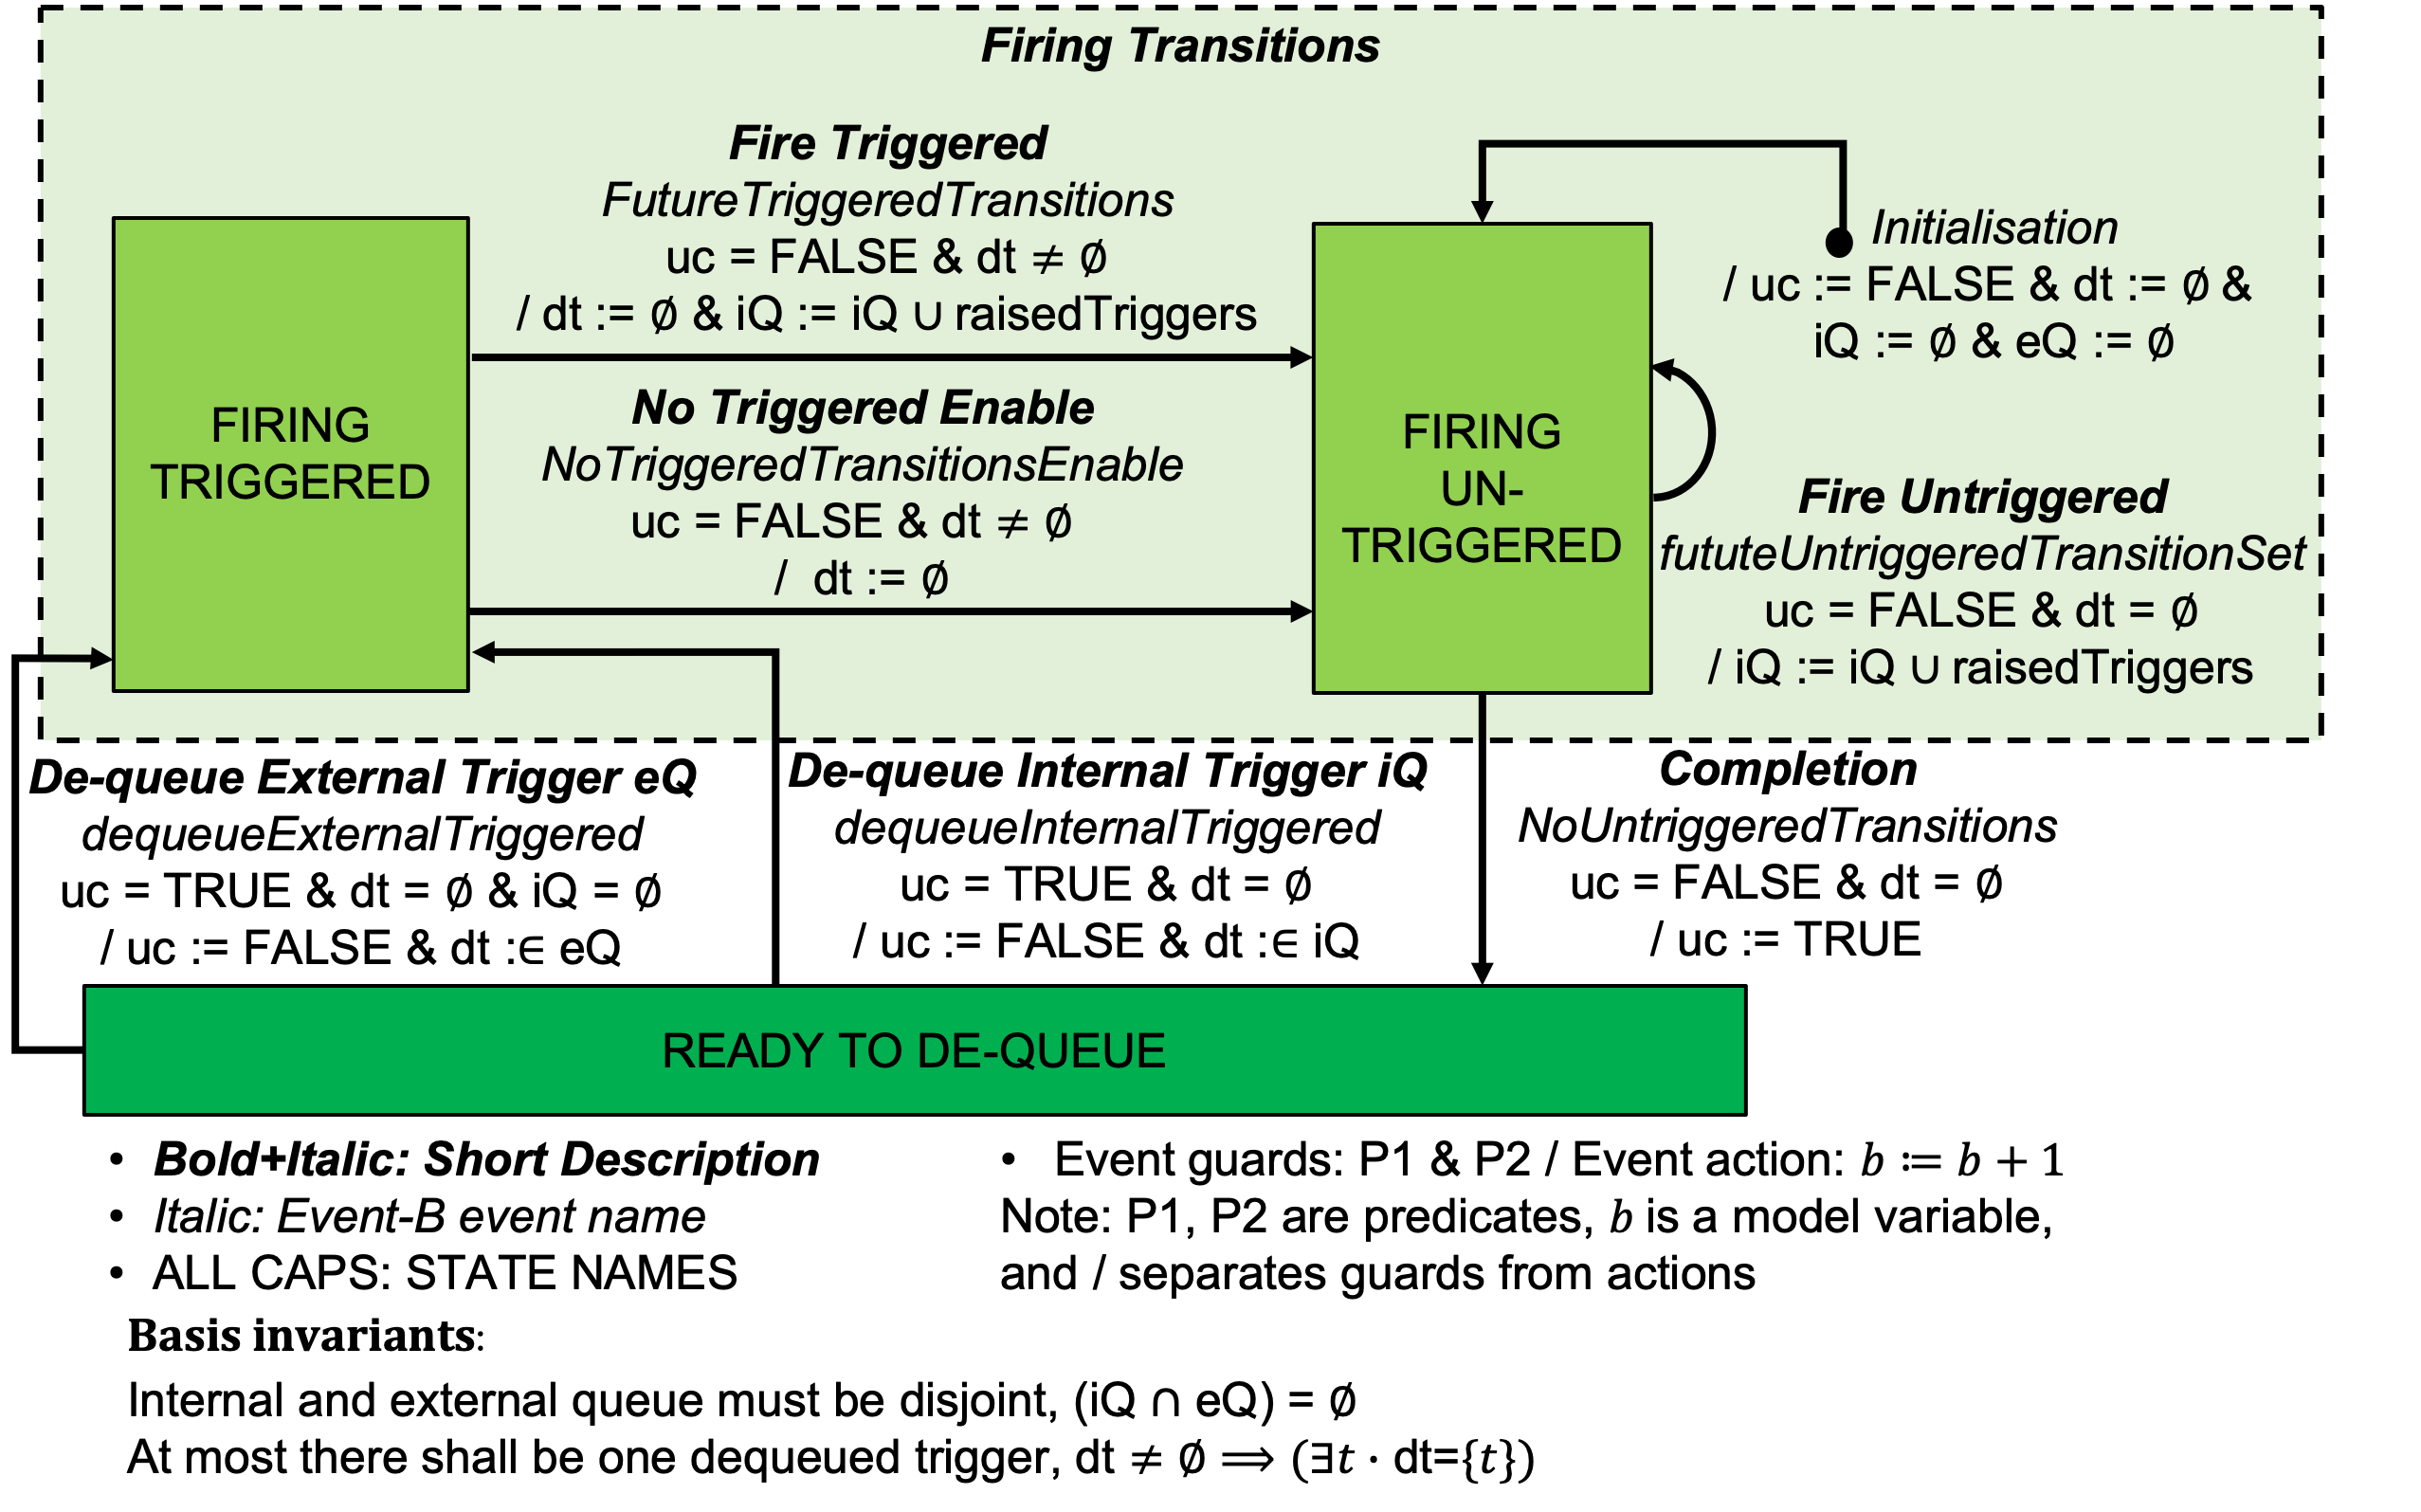
\includegraphics[width=0.90\textwidth, trim=30 50 60 0]{figures/Picture6.png}
	\caption{Abstract representation of run to completion basis}
	\label{fig:basis}
	\vspace{-.4cm}
\end{figure}

The specification of this basis consists of an \EVENTB \emph{context} and \emph{machine} that are the same for all input models and are refined by the specific output of the translation.  
The basis context, shown in listing \ref{lst:BasisContext}, introduces a set of all possible triggers, |SCXML_TRIGGER| which is partitioned into internal and external triggers 
(e.g |FutureInternalTrigger| and |FutureExternalTrigger| respectively), 
some of which will be introduced in future refinements. 
At each refinement these trigger sets are further partitioned to introduce more concrete triggers, 
leaving a new abstract set to represent the remaining triggers yet to be introduced. 

The context also models \emph{sequences} of triggers as a data type to be used for the trigger queues.
Our initial work modelled queues abstractly as sets of triggers which was adequate for most verification purposes but does not enforce fairness on trigger consumption~\cite{MoSnHo18,MoSnHo-ABZ2020,detect2020}. 
Hence we were forced to introduce fairness assumptions regarding trigger consumption in order to verify liveness properties.
In this paper we introduce sequences to properly model the trigger queues which are an implementation of this fairness property. 
Note that the queue also enables the same trigger to be raised twice in the queue which was not possible in a set.
The constant |Seq| returns the set of all possible sequences of a given subset of triggers and is defined using lambda calculus.
Constant functions are also defined for the usual operations on sequences: 
\emph{length} of a given sequence, 
\emph{append} a trigger to the end of a sequence to give a new sequence, 
\emph{concat}enate two sequences to give a new sequence, 
return the trigger at the \emph{head} of a sequence, 
return the sequence that makes up the \emph{tail} of a sequence and 
return the \emph{content} (set of triggers) involved in a sequence. 
The Basis context also defines several theorem properties about sequences that are needed to discharge proof obligations.
These are omitted from Listing~\ref{lst:BasisContext} for brevity.

\ColinInlineComment{I changed the comments to a command in order to get them to align.  Is there a better way? }
\newcommand*{\Comment}[1]{\color{green!50!black}\hfill\makebox[0.6\textwidth][l]{#1}}%

 \begin{lstlisting}[caption={Abstract basis context},label={lst:BasisContext}, language=Event-B, tabsize=8, escapechar=€, frame=single, basicstyle=\rmfamily\scriptsize, belowskip=-2.0 \baselineskip, float=t]
 context
 	basis_c 	€\Comment{// (generated for SCXML)}€
 sets
 	SCXML_TRIGGER	 €\Comment{// all possible triggers}€
 constants
 	FutureInternalTrigger	€\Comment{// all possible internal triggers}€
 	FutureExternalTrigger	€\Comment{// all possible external triggers}€
 	Seq							€\Comment{// return all possible sequences of given set of triggers}€
 	Seq_length					€\Comment{// return the length of a sequence of triggers}€
 	Seq_append					€\Comment{// return the result of appending trigger to a sequence}€
 	Seq_concat					€\Comment{// return the concatenation of two sequences of triggers}€
 	Seq_head					€\Comment{// return the trigger at head of a sequence of triggers}€
 	Seq_tail					€\Comment{// return the sequence at tail of a sequence of triggers}€
 	Seq_content					€\Comment{// return the set of triggers in a sequence of triggers}€
 	InternalQueueType			€\Comment{// type of internal queues}€
 	ExternalQueueType			€\Comment{// type of external queues}€
 	
 axioms
 	partition(SCXML_TRIGGER, FutureInternalTrigger, FutureExternalTrigger) 
 	Seq = (λT · T ⊆ SCXML_TRIGGER ∣ {n, s · n ∈ ℕ ∧ s ∈ 0 ‥ n − 1 → T ∣ s})
 	Seq_length = (λs · s ∈ Seq(SCXML_TRIGGER) ∣ card(s))
 	Seq_append = (λ s ↦ t · s ∈ Seq(SCXML_TRIGGER) ∧ t ∈ SCXML_TRIGGER ∣ 
 		{i↦v ∣ i ∈ 0 ‥ Seq_length(s) ∧ (i < Seq_length(s) ⇒ v = s(i)) ∧ (i = Seq_length(s) ⇒ v = t) } )
	Seq_concat = (λ s1 ↦ s2 · s1 ∈ Seq(SCXML_TRIGGER) ∧ s2 ∈ Seq(SCXML_TRIGGER) ∣ 
		{i↦v ∣ i ∈ 0 ‥ Seq_length(s1) + Seq_length(s2) − 1 ∧ (i < Seq_length(s1) ⇒ 
									v = s1(i)) ∧ (i ≥ Seq_length(s1) ⇒ v = s2(i − Seq_length(s1))) } )
	Seq_head = (λs · s ∈ Seq(SCXML_TRIGGER) ∧ s ≠ ∅ ∣ s(0))								
	Seq_tail = (λs· s∈Seq(SCXML_TRIGGER) ∧ s≠∅ ∣ {i↦v ∣ i∈0‥Seq_length(s)−2 ∧ v=s(i+1)} )	
	Seq_content = (λs · s ∈ Seq(SCXML_TRIGGER) ∣ ran(s))
	InternalQueueType = Seq(FutureInternalTrigger)
	ExternalQueueType = Seq(FutureExternalTrigger)
 end
 \end{lstlisting}	

Each of the transitions in the basis (see Figure~\ref{fig:basis}) represents an abstract event of the basis machine (Listing~\ref{lst:BasisMachine}) that describes the generic behaviour of models under a run to completion semantics.
These events provide an abstraction that defines the altering of trigger queues and completion flag. 
\EventB refinement rules prohibit new events from modifying abstract variables (i.e. new events refine `skip').
Hence, since \SCXML transitions need to modify the trigger queues etc., used to capture the \SCXML run to completion semantics, all events generated by translation of the specific \SCXML model,  must refine abstract events introduced for this purpose in the basis.
The basis machine also declares variables that correspond to the currently dequeued trigger,  |dt|, 
the queue of internal triggers raised by actions within the model, |iQ|, 
the queue of external triggers raised by the environment, |eQ|,
and a flag, |uc|, that signals when a run to completion macro-step has been completed 
(no un-triggered transitions are enabled). 
Note that, for convenience, the currently dequeued trigger, |dt|, is modelled as a singleton set which may be empty (i.e. consumed) or contain the single trigger to be consumed.

The trigger queues and dequeued trigger are initialised to empty and |uc| is set to |FALSE| so that any enabled un-triggered transitions are dealt with via the |futureUntriggeredTransitionSet| event when the system first starts (see Listing~\ref{lst:scxml-r2c}).
This will subsequently enable completion and reset the |uc| flag to |TRUE|.
The abstract event |futureRaiseExternalTrigger| represents the raising  of an external trigger (not shown in figure~\ref{fig:basis}).    
After completion, a queued trigger can be prepared for consumption by moving it to the dequeued trigger, |dt|.
Internal triggers have a higher priority, since the external trigger queue is only dequeued if the |iQ| is empty (see |dequeueExternalTriggered| and |dequeueInternalTriggered| in Figure~\ref{fig:basis}).
The abstract event |futureTriggeredTransitionSet| represents a combination of parallel transitions that may be simultaneously triggered by the dequeued trigger, |dt|.
When the actual example \SCXML is translated, a separate refinement of this abstract event will be generated for each subset of the set of parallel transitions that could fire in parallel in order to cater for all possibilities of enablement, however, as the model is refined some combinations may be eliminated as the guards are strengthened.
This approach to generating an event for each possible combination of each set of transitions that could fire in parallel is needed because of the batch enabling semantics of the SCXML run to completion (see Section~\ref{sec:scxml}).
The actions of these transitions may also raise triggers of their own in the internal trigger queue |iQ|.


Completion of triggered and untriggered transitions may be non-deterministically premature to allow future refinements to strengthen the guards of transitions (i.e. to disable them resulting in an earlier completion).
In the process of refining a model, a designer takes advantage of this non-determinism in the abstraction by adding nested sub-states and explicit guards to transitions. 
When a refinement level is reached where the designer wants to enforce a requirement (i.e. prevent it being bypassed by a non-deterministic completion), the model needs to be \emph{finalised} (see Section~\ref{sec:translation} for more on finalisation). 
The \SCXML translation tool will then automatically strengthen the guards of events |noTriggeredTransitionsEnabled| and |noUntriggeredTransitionsEnabled|, to ensure that the run to completion sequence is not interrupted by non-deterministic behaviour. 
To do this we need to guard completion so that it cannot happen while any relevant transition is still enabled.
To finalise a triggered transition, the guard of |noTriggeredTransitionsEnabled| is strengthened by adding the conjunction of the negated guards of all transitions that can fire in parallel with the transition being finalised.
%(To fire in parallel a transition must be in a parallel region of the state-chart and be triggered by the same trigger).
Similarly, to finalise an untriggered transition, the guard of |noUntriggeredTransitionsEnabled| is strengthened by adding the conjunction of the negated guards of all untriggered transitions that can fire in parallel.
It may seem that finalisation could cause an unmanageable explosion of guards.
However, to fire in parallel, transitions must be contained in parallel regions and also be enabled by the same trigger (or be un-triggered).
In practice, since most systems do not contain many parallel regions, the number of transitions that can fire in parallel is limited.
Transition finalisation can be left until it is needed for the proof of a particular property and does not generate any new proof obligations since adding guards is a trivial refinement step.
Finalisation is also needed in order to remove non-deterministic behaviours when the model is animated for validation purposes.

% The basis machine declares variables 
% that correspond to the triggers present in the queue at any given time, and a flag, |SCXML_uc|, that signals when a run to completion macro-step has been completed (no un-triggered transitions are enabled). 
% After initialisation, both trigger queues are empty and |SCXML_uc| is set to |FALSE| so that un-triggered transitions are dealt with. 
% The basis machine provides events that describe the generic behavior of models that follow the run to completion semantics in terms of altering the trigger queues and completion flag.
% Since new events introduced in a refinement cannot modify existing variables, all future events generated by translation of the specific \SCXML model, will refine these abstract events.
% The abstract event, |SCXML_futureRaiseExternalTrigger| represents the raising of an external trigger (this transition is not shown in the diagram).    
% The abstract event, |SCXML_futureInternalTransitionSet| represents a combination of transitions that are triggered by an internal trigger. 


% The guards of this event ensure prior completion of the previous macro-step. 
% A similar event, |SCXML_futureExternalTransitionSet| (not shown) represents a combination of transitions that are triggered by an external trigger and has the additional guard that the internal trigger queue is empty.
% These two triggered transition events reset the completion flag to ensure that any un-triggered transitions that may have become enabled have a chance to fire next.
% The abstract event |SCXML_futureUntriggeredTransitionSet| represents a combination of transitions that are un-triggered and may only be fired when the completion flag is unset (FALSE).
% It leaves the completion flag unset in case further combinations of un-triggered transitions are enabled.
% All three of these transition events also allow for raising a non-deterministic set of internal triggers.
% A final abstract event, |SCXML_completion|, sets the completion flag (TRUE) if it is not already set. At this abstract basis level, this is non-deterministically fired since we do not yet have any detail of what needs to be completed.




 \begin{lstfloat}[!tb]
 \begin{lstlisting}[caption={Abstract basis machine}, label={lst:BasisMachine},language=Event-B, escapechar=€, frame=single, basicstyle=\rmfamily\scriptsize, belowskip=-2.0 \baselineskip]
 MACHINE	basis	   €\Comment{//   (generated for SCXML)}€
 SEES    	basis_ctx
 VARIABLES
 €~~€	iQ	   €\Comment{//   internal trigger queue}€
 €~~€	eQ	   €\Comment{//   external trigger queue}€
 €~~€	uc	   €\Comment{//   run to completion flag}€
 €~~€	dt	   €\Comment{//   dequeued trigger for this run}€
 INVARIANTS
 €~~€	iQ ∈ InternalQueueType	   	€\Comment{//   internal queue}€
 €~~€	eQ ∈ ExternalQueueType	   	€\Comment{//   external queue}€
 €~~€	uc ∈ BOOL	   				€\Comment{//   completion flag}€
 €~~€	dt ⊆ SCXML_TRIGGER	   		€\Comment{//   dequeued trigger}€
 €~~€	dt≠∅ ⇒(∃t·dt={t})			€\Comment{//   at most one dequeued trigger}€
 EVENTS
 	INITIALISATION   €\Comment{// queues empty, completion false, no dequeued triggers}€
 			iQ, eQ, uc, dt ≔ ∅,	∅, FALSE, ∅  
 	END

 	futureRaiseExternalTrigger      	   €\Comment{//basis of future event to raise an external trigger}€
 		ANY 	raisedTrigger	WHERE raisedTrigger ∈ FutureExternalTrigger
 		THEN	eQ≔append(eQ ↦ raisedTrigger)
 	END

 	dequeueInternalTrigger      	   €\Comment{//event to dequeue an internal trigger}€ 
 		WHEN	iQ≠∅ & dt=∅ & uc=TRUE 
 		THEN	dt, iQ, uc ≔ {head(iQ)}, tail(iQ), FALSE
 	END

 	dequeueExternalTrigger      	   €\Comment{//event to dequeue an external trigger}€ 
 		WHEN	eQ≠∅ & dt=∅ & uc=TRUE & iqQ∅
		THEN	dt, eQ, uc ≔ {head(eQ)}, tail(eQ), FALSE
 	END

 	futureTriggeredTransitionSet      	€\Comment{//basis of future event representing triggered transitions}€
 		ANY trigger, raisedTriggers WHERE trigger ∈ dt & uc = FALSE & raisedTriggers ∈ Seq(FutureInternalTrigger)
 		THEN	dt, iQ ≔ ∅ , concat(iQ↦raisedTriggers)
 	END

 	noTriggeredTransitionsEnabled      	€\Comment{//event to fire when no triggered transitions enabled}€ 
 		WHEN 	uc=FALSE & dt≠∅
 		THEN	dt ≔ ∅
 	END

 	futureUntriggeredTransitionSet      €\Comment{//basis of future event representing untriggered transitions}€
 		ANY	raisedTriggers	WHERE	uc=FALSE & dt=∅ & raisedTriggers∈Seq(FutureInternalTrigger)
 		THEN iQ ≔ concat(iQ↦raisedTriggers)
 	END

 	noUntriggeredTransitionsEnabled      €\Comment{//event fired when no untriggered transitions enabled}€
 		WHEN	uc=FALSE & dt=∅
 		THEN	uc ≔ TRUE
 	END
 END
 \end{lstlisting}
 \end{lstfloat}

% \begin{lstfloat}[!tb]
% \begin{lstlisting}[caption={Event-B event corresponding to internal triggered transition to \textbf{Wait50ms} state in refinement level 1 shown in Fig.~\ref{fig:ASIC}}, label={lst:SecBotMach0},language=Event-B, escapechar=|, frame=single, belowskip=-2.0 \baselineskip]
% spi_done__InitialiseSensor_Wait50ms:	
% refines SCXML_futureInternalTransitionSet 
% any SCXML_it SCXML_raisedTriggers where
% SCXML_it  ∈ SCXML_iq 
% SCXML_uc = TRUE
% SCXML_raisedTriggers ⊆ SCXML_FutureInternalTrigger
% InitialiseSensor = TRUE
% SCXML_it = spi_done  	//trigger for this transition |\label{line:defTrigger}|
% then
% SCXML_uc ≔ FALSE
% SCXML_iq ≔ (SCXML_iq ∪ SCXML_raisedTriggers) ∖ {SCXML_it}
% InitialiseSensor ≔ FALSE
% Wait50ms ≔ TRUE
% end
% \end{lstlisting}
% \end{lstfloat}

%%% Local Variables:
%%% mode: latex
%%% TeX-master: "../main"
%%% End:

% !TEX root = ../main.tex


\section{Translation to Event-B}

\emph{Describe how we enhance SCXML with `umlb' attributes (inc. refinement levels) and translate into UML-B state-machines.}
% !TEX root = ../main.tex
\section{Description of the Sample Application}
\label{sec:descr-sample-appl}

To illustrate the development and analysis process of a design using the previously described 
state-chart semantics, we will discuss a quadrotor helicopter or quadrotor application similar to 
the one presented by Syriani et al.~\cite{Syriani_2019}. 
The application will focus on the incremental design of some of the drone's required functionality.
The constructed model must obey state-chart refinement rules listed in Section~\ref{sec:intro}, these rules are proven within the Rodin tool.
The structure of the state-chart for this model at each subsequent abstraction level restricts further the development of the model to refinements that obey the rules. 
This will allow us to prove properties of the model in a very strategic fashion, as properties proven of early abstraction levels are preserved in later refinements.

The initial abstraction and first refinement of the model, shown in Figure~\ref{fig:drone1}, capture the basic functionality of the drone. 
The abstract model is shown in blue; the model's initial state is |OFF| and as a result of the |on| and  |toTakeoff| external triggers it transitions to the |START| and |OPERATIONAL| states respectively\footnote{Transitions in Figures~\ref{fig:drone1}--\ref{fig:drone4} are labeled with trigger names
(e.g. toTakeoff, toFly) not with event names as it is in \UMLB.}. 
The drone reacts to the |off| external trigger by shutting down and subsequently transitioning to the |OFF| state.
The first refinement is constructed using \emph{Rule C}, which adds details within the |OPERATIONAL| state (gray states in Figure~\ref{fig:drone1}).
Within the |OPERATIONAL| state the drone will transition to |FLY| or |DESCEND| after the internal trigger |toFly| or |toLand| is raised, respectively. 
In refinement level one, these internal triggers are raised non-deterministically in the system by functionality not currently defined.
As additional details are incorporated into the model in later refinements some of that non-determinism is 
removed and replaced by transitions with actions that raised the previously defined internal triggers.
A further external trigger, |landed|, directs the system to progress to the |LANDED| state.
It should be noted that this abstraction of the drone model includes a transition from |TAKEOFF| to |DESCEND| (dashed transition in Figure~\ref{fig:drone1}). 
This allows for the drone to respond to a |toLand| trigger if it encounters some problems while in the |TAKEOFF| state.
Syriani et al.~\cite{Syriani_2019} introduces this transition in later refinements under Rule 8 \emph{path refinement rule}. 
This rule is inconsistent with our rules of refinement as it results in a concrete event with no corresponding behavior in the abstraction.

% \begin{figure}[!h]
\begin{figure}[]
	\vspace{-.4cm}
	\centering
	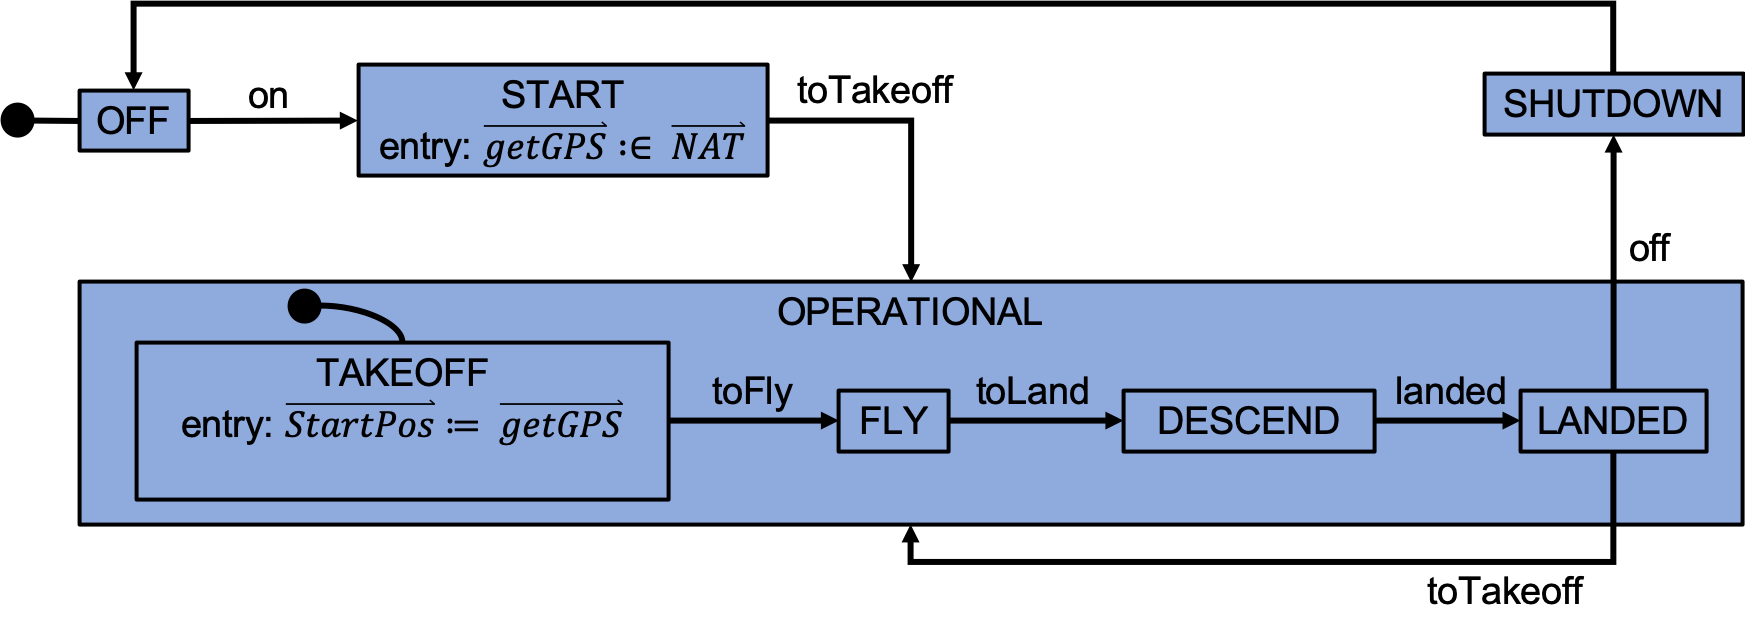
\includegraphics[width=0.90\textwidth, trim=0 40 0 0]{figures/Picture1.png}
	\caption{State-chart of drone application. Abstract level including only generic start/shutdown behavior (shown in blue). The first refinement introducing main operational sub-states, is shown in gray. }
	\label{fig:drone1}
	\vspace{-.4cm}
\end{figure} 


% Figure~\ref{fig:drone2} shows the first refinement of the model, as we refine the parent state |TAKEOFF|
% by introducing child states and new model variables, similar to 
% Rule 2 \emph{basic-to-or state rule} defined by Syriani et al.~\cite{Syriani_2019}
% As part of this refinement we introduced an untriggered transition responsible for 
% raising the |toFly| internal trigger, and therefore removed some of the non-determinisms in the abstraction.

% \begin{figure}[!h]
% 	\centering
% 	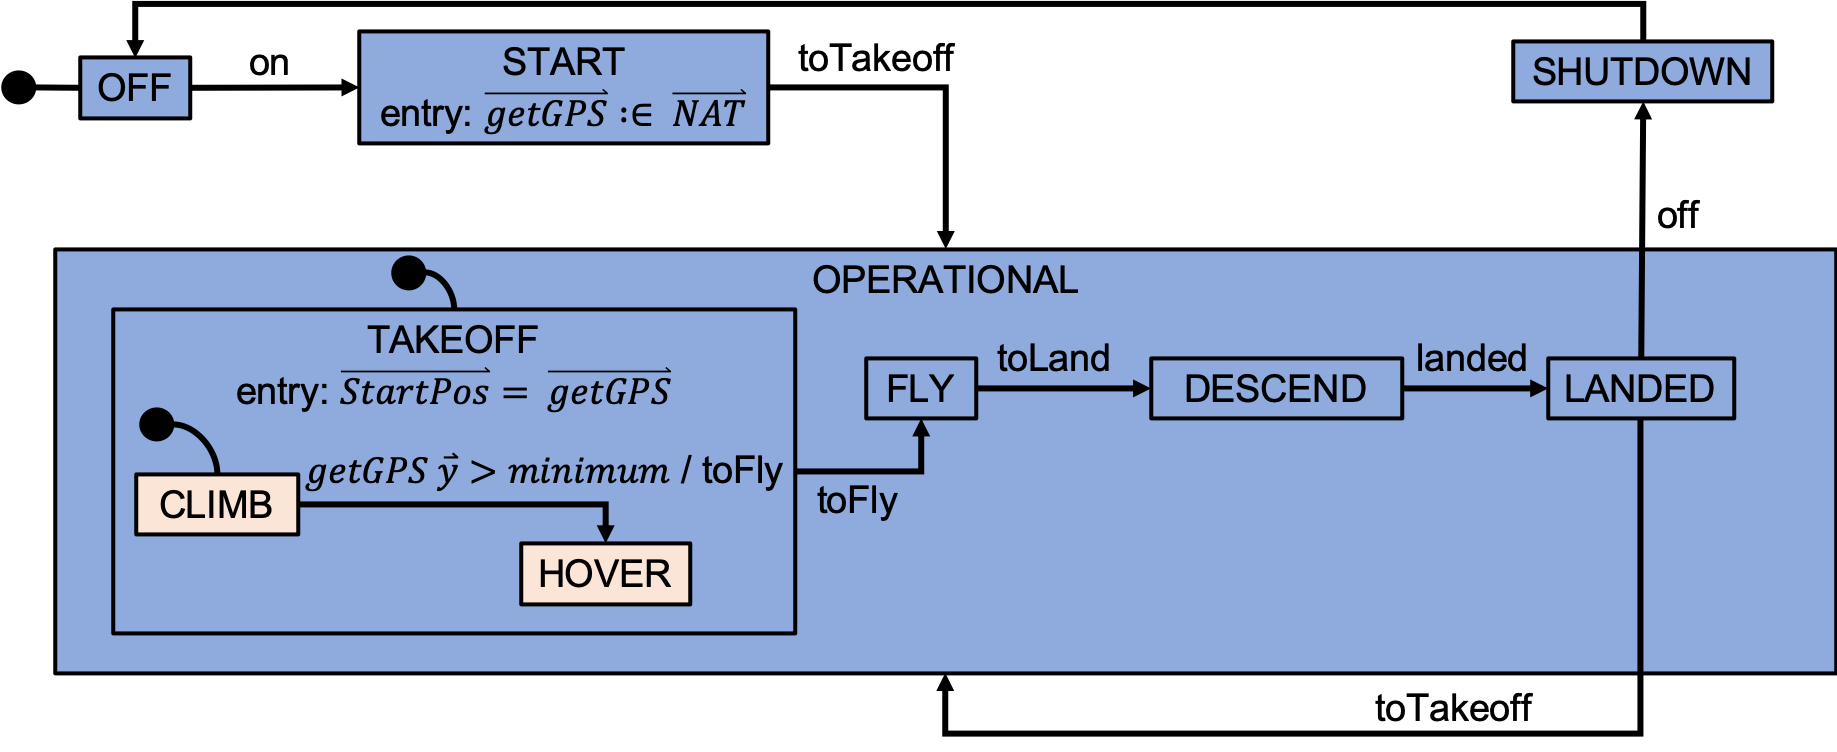
\includegraphics[width=0.95\textwidth]{figures/Picture2.png}
% 	\caption{State-chart of drone application. Refinement level introducing details for take off.}
% 	\label{fig:drone2}
% \end{figure} 
% \begin{figure}[!h]

\begin{figure}[]
	\centering
	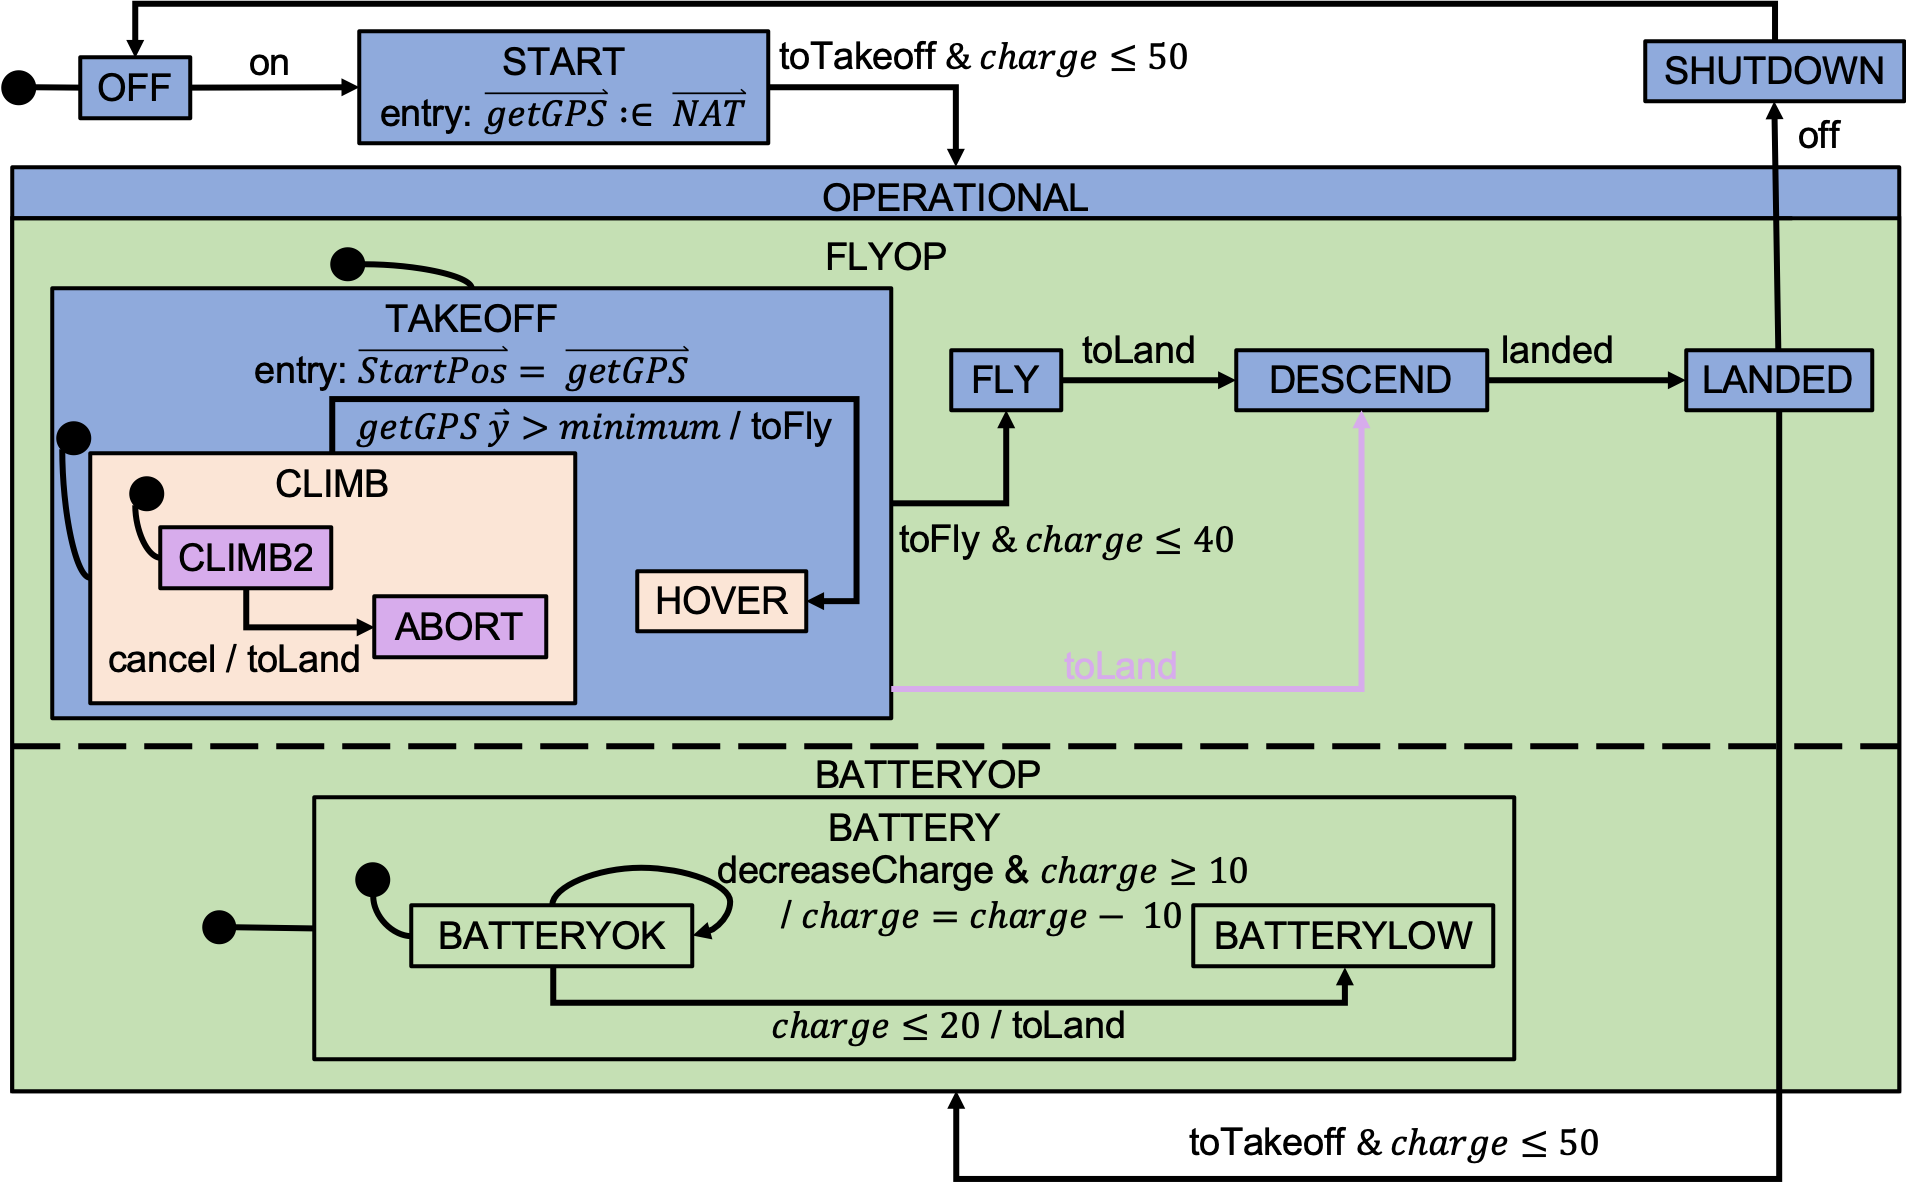
\includegraphics[width=0.90\textwidth, trim=0 30 0 0]{figures/Picture5.png}
	\caption{State-chart of drone application. 
		2nd refinement for battery monitoring functionality (shown in green).
		3rd refinement introducing details for take off (shown in beige).
		4th refinement level to allow cancelling during take-off (shown in lilac).}
	\label{fig:drone4}
\end{figure} 

Figure~\ref{fig:drone4} builds on Figure~\ref{fig:drone1} to show three more refinements to the drone model. 
% Figure~\ref{fig:drone4} shows two subsequent refinements to the drone model.
The second refinement (shown in green in Figure~\ref{fig:drone4}) extends the capabilities within |OPERATIONAL| by using \emph{Rule C} to make it a parallel state that controls flying and battery related functionality. 
This is the same as Rule 4 \emph{and-state rule} defined by Syriani et al.~\cite{Syriani_2019}.
The charge within the drone battery is monitored by the parallel |BATTERYOP| state. 
A new ancillary variable, |charge|, is introduced to keep track of the amount of charge left in the drone.
It is decreased by a self-transition on state |BATTERYOK| in response to an external trigger |decreaseCharge|. 
%As part of this design stage we introduce a requirement to constrain drone flying operation to a battery charge of at least 20\% capacity.
If the battery monitor works correctly we would expect the battery charge to have at least 20\% capacity while in the state |BATTERYOK|.
This can be expressed as an invariant property:
\begin{center}
	|(BATTERYOK = TRUE) => charge > 20|\% .
\end{center}
When the monitored charge drops to 20\% or less, the |BATTERY| state-chart raises the internal trigger |toLand|, which will cause a reaction in the |FLYOP| start-chart to bring it out of |TAKEOFF| or |FLY| and into |DESCEND| (hence removing some of the non-determinism concerning where |toLand| is raised).
While in the |TAKEOFF| state we would expect the battery monitor to be in the |BATTERYOK| state or to have raised a |toLand| trigger.
\begin{center}
	|(TAKEOFF = TRUE) => (BATTERYOK = TRUE ∨ toLand)|~.
\end{center}
%The aforementioned trigger, is raised non-deterministically by some unspecified internal functionality .
%Our state-chart semantics supports transition refinement, which allows us to modify previously defined transitions, by adding guards \emph{Rule A} and/or actions \emph{Rule B} that modify new variables that contribute implementation details to the model. 
To ensure the drone only enters |TAKEOFF| or |FLY| with enough battery power we strengthen the guards of transitions to the |FLY| and |TAKEOFF| states (\emph{Rule A}).
We will discuss how these state invariant properties are verified in Section~\ref{sec:verificationSafety}.

% \begin{figure}[!h]
% 	\centering
% 	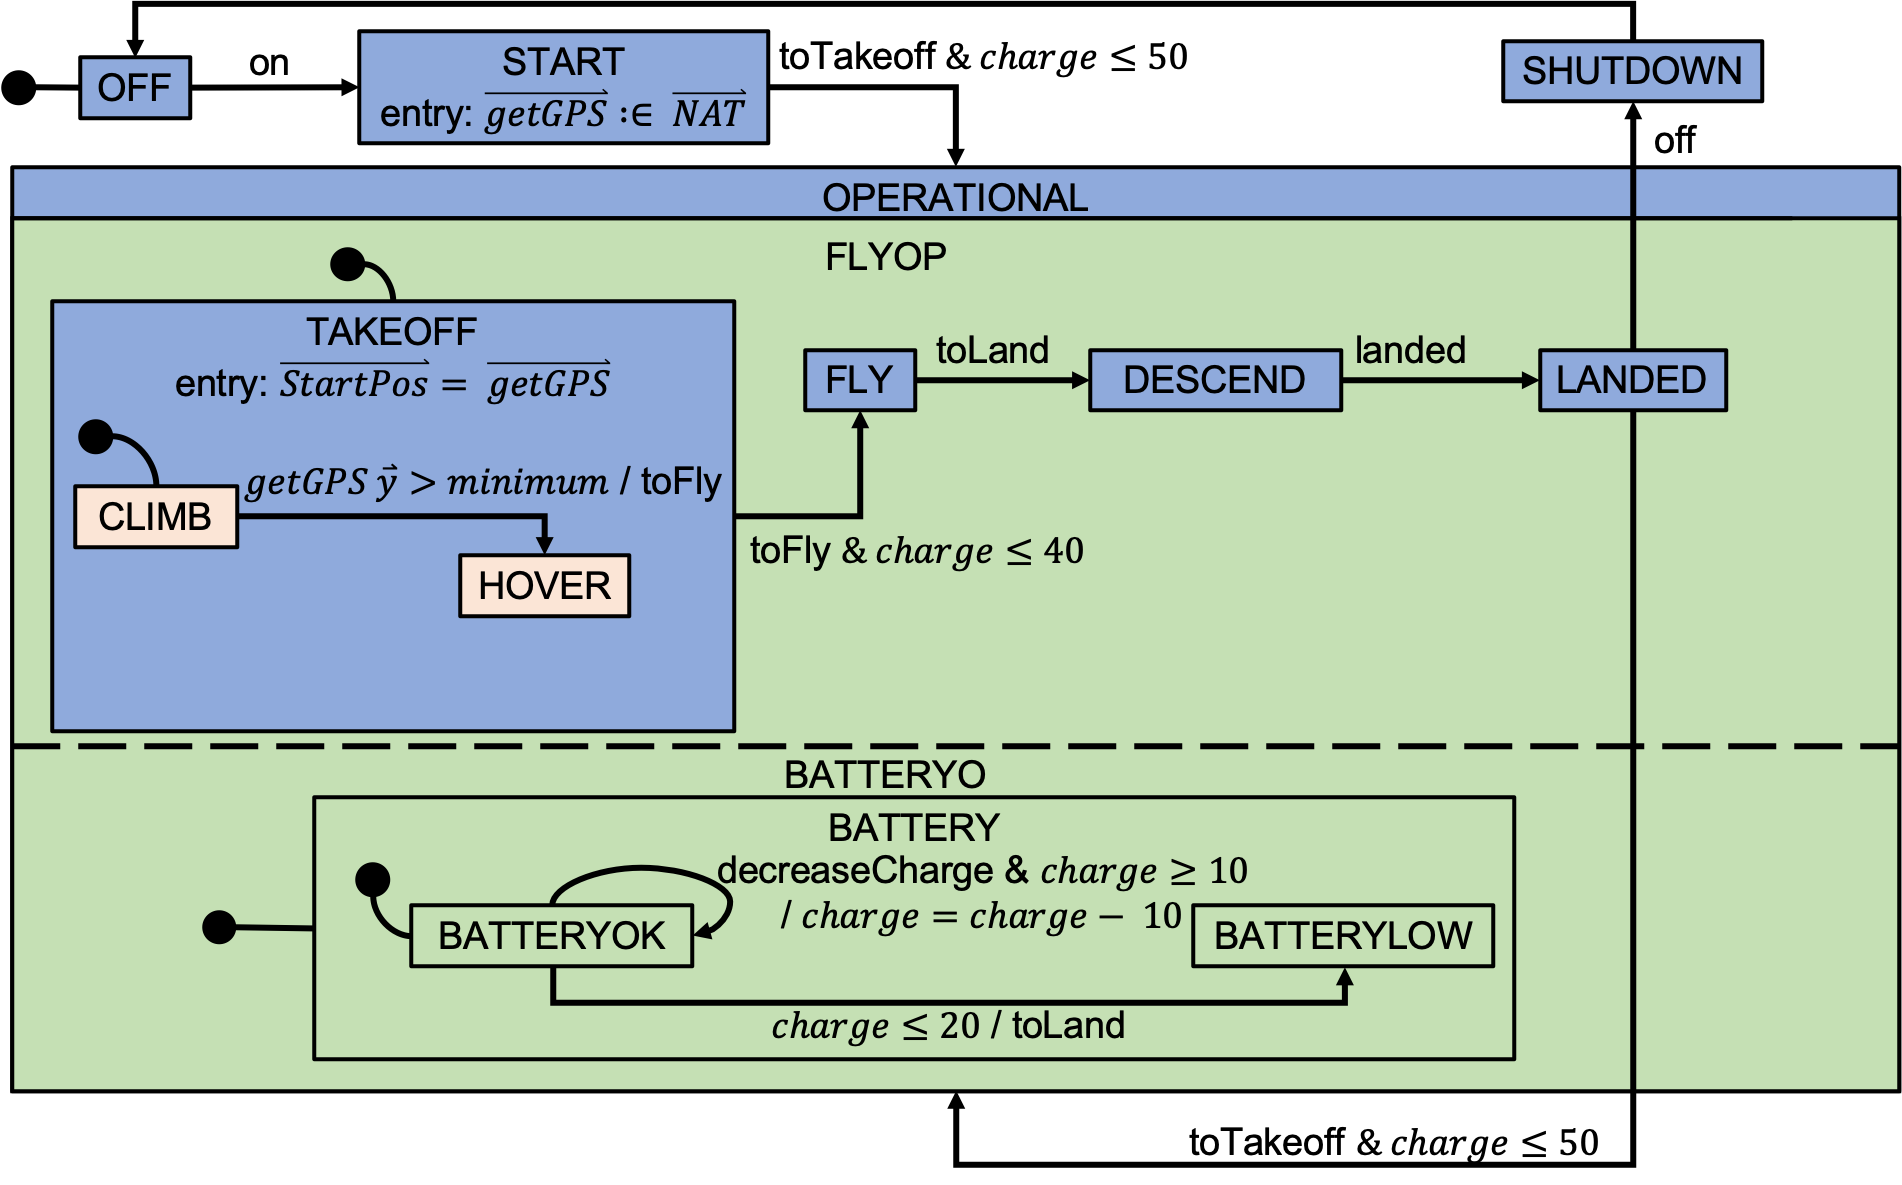
\includegraphics[width=0.95\textwidth]{figures/Picture3.png}
% 	\caption{State-chart of drone application.Refinement level for descending capabilities}
% 	\label{fig:drone3}
% \end{figure} 

The third refinement of the model (shown in beige) refines the state |TAKEOFF| by applying \emph{Rule B and C}. 
Under these rules we introduce child states and new model variables, similar to Rule 2 \emph{basic-to-or state rule} defined by Syriani et al.~\cite{Syriani_2019}
As part of this refinement we introduced an untriggered transition responsible for raising the |toFly| internal trigger, and therefore removed some of the non-determinisms concerning this trigger.

The fourth refinement of the drone model (shown in lilac) uses \emph{Rule C} to introduce additional implementation details to 
allow a take-off to be cancelled in response to an external trigger |cancel|.
%ensure that under special 
%circumstances (e.g. sensing of adverse environment or unexpected battery dropped) the drone is able 
%to circumvent flying and proceed to an emergency landing. The previously described requirement can be
%expressed as
%\begin{center}
%  |(TAKEOFF = TRUE) => (BATTERYOK = TRUE ∨ toLand)|~.
%\end{center}
%To implement this new capability in the design the internal trigger |cancel| is introduced.
%The internal trigger |cancel| can be raised non-deterministically by some sensing capability, 
%the details of which are not currently implemented. 
If the trigger is raised, the climbing process must be aborted and the drone descending sequence shall start. 
This refinement level is done differently to Syriani et al.~\cite{Syriani_2019}, which follows Rule 7 \emph{state extension rule}. 
The aforementioned rule requires a data remapping of the abstract states |TAKEOFF|, |CLIMB| and |HOVER|, which should be distinct from the states in this  refinement, as the state |ABORT| is introduced.
In contrast, we implement this refinement using a rule similar to Syriani et al.'s  Rule 2 \emph{basic-to-or state rule}, which introduces the concrete states |CLIMB2| and |ABORT| to the abstract state |CLIMB|.


% Syriani et al. refinement rules
% Rule 1 \emph{action rule}
% Rule 2 \emph{basic-to-or state rule}
% Rule 3 \emph{or-to-and state rule}
% Rule 4 \emph{and-state rule}
% Rule 5 \emph{transition rule}
% Rule 6 \emph{fork rule}
% Rule 7 \emph{state extension rule}
% Rule 8 \emph{path refinement rule}

% Event-B refinement rules
% https://www3.hhu.de/stups/handbook/rodin/current/html/generated_proof_obligations.html
% guard strengthening
% action simulation
% equality of a preserved variable
% guard strengthening (merge)
% well definedness of a witness
% feasibility of witness
% decreasing of variant

%%% Local Variables:
%%% mode: latex
%%% TeX-master: "../main"
%%% End:

% !TEX root = ../main.tex

\section{State-chart Refinement}
\label{sec:scref}

Our system includes three refinement rules.

\begin{enumerate}
\item Guard conditions on a transition can be strengthened; 
this can done by adding textual guards to the transition, or
changing the source of the transition to a nested state.
\item Transitions can have additional actions, provided they do not
  modify variables appearing in the abstraction; this can be 
  accomplished by adding textual action to the transition 
  or by changing the target to nested state.
\item A state-chart can be embedded within a state of another
  state-chart -- sometimes called hierarchical composition or
  hierarchical refinement.
\end{enumerate}

Via the translation explained in Section~\ref{sec:translation}, these rules
rely on the usual \EventB proof obligations to ensure that they do
indeed yield refinements in the \EventB semantics.

If an \EventB model |B| can be shown (via the construction rules of
the \EventB language as well as the proof obligations) to refine
another \EventB model |A|, then we know that every behavior of |B| is
also a behavior of |A|. This definition yields a useful principle of
preservation of safety -- if we can show that a bad thing never
happens in |A|, then we can add detail via refinements in |B|, knowing
that the bad thing will continue to never happen in |B|. That is,
\EventB refinements preserve safety properties in the sense
of~\cite{lamport1977proving}. This makes refinement a useful technique
in developing safety-critical systems: one can analyze a simpler
abstract model for critical safety properties and then add detail to
the model via refinements, secure in the knowledge that the safety
properties will be preserved.

\EventB refinements have also been shown to preserve some liveness
properties, under certain conditions~\cite{hoang2016ltl}.

Although the autonomous drone example in this paper is based on the
example described in~\cite{Syriani_2019}, the definition of refinement
used in that work is quite different from our own. This forces some
differences in our refinement rules and consequently the way the
example is developed. For example, the transition triggered by |toLand| 
(see ~\ref{fig:drone4} transition from |TAKEOFF| to |DESCEND|) 
adds new behaviour.
In~\cite{Syriani_2019} ``refinement'' is a
transformation of the model which preserves reachability of a state
with respect to sequences of inputs. This guarantees that a refinement
in their system will include all the behaviors of the abstraction,
while possibly adding others. While this notion of refinement seems
useful in certain contexts, unlike refinement in \EventB it does not
guarantee preservation of safety properties. Therefore it should be
considered less suited to development of safety-critical systems.


% !TEX root = ../main.tex


\section{Verification of Safety Properties}
\label{sec:verificationSafety}

\todo{Merge the 2 verification section into one. And just the general form of the properties that can discharge automatically}
In a state-chart model we naturally wish to verify properties |P|, about other parallel statechart regions and auxiliary data, that are expected to hold true in a particular state |S|.
Hence, all of the safety properties that we consider are of the form: |S=TRUE ⇒ P|, where the antecedent is implicit from the containment of |P| within |S|.
%
%There are two kinds of properties that we might want to verify in an \SCXML state-chart;
%1) properties concerning the values of auxiliary data maintained by the system and 
%2) constraints about the state of another parallel state-chart region.

\SCXML models represent components that respond to received triggers and are not perfectly synchronised with changes in the monitored properties. 
Hence, |P| may be temporarily violated until the system responds by leaving the state |S| in which the property is expected to hold.
To cater for this we express |P| in a modified form |P'| that allows time for the response to take place.
There are two forms of reaction that can be used to exit |S|; 
a) an untriggered transition, or 
b) a transition that is triggered by an internally raised trigger.
For a), the modified property |P'| becomes |P ∨| \emph{untriggered transitions are not complete}, 
and for b) |P'| becomes |P ∨| \emph{trigger} |t| \emph{is in the internal queue or dequeued}
(where |t| is the internal trigger raised when the violation of |P| is detected).

%Not sure the following is true so removed it..
%For properties about the value of auxiliary data, untriggered transitions appear to be more suited because, in this case, there is unlikely to be a natural place to raise an internal trigger when the appropriate conditions arise.
%For properties about the state of a parallel region either reaction could be used depending on whether the system detects the violation in the state that contains P of the state that P refers to.

\todo{Insert a general form of the sort of properties we can verify and discuss} 
% In this section we illustrate a typical example of the type of properties that we imagine could be verified in a reactive \SCXML system.
% All of the proof obligations are automatically discharged for our example.
% Since our models are strictly structured and proof obligations will always have this common form, we are optimistic that proofs will always discharge automatically.
% We model the safety property features at an early level of refinement where the models are relatively simple, so that the validity of verification conditions is clear. 
% Detail is then added in later refinements which are proven (automatically) to preserve the previously verified safety properties.
% In our example, some auxiliary data is monitored by one state-chart region and while a parallel region refers to the state of the monitoring region. 
% Hence the reaction consists of an un-triggered transition in the monitoring region which sends an internal trigger to the other region when it leaves the desired monitor state.

% For our drone model, the safety property that we wish to verify is that the control system does not continue to take off or fly if the battery charge drops below a certain threshold (say 21\%). 
% By refinement level 1 we have developed the drone's state to the point where we distinguish the |TAKEOFF| and |FLY| states (Figure~\ref{fig:drone1}).
% In refinement level 2 we therefore introduce the battery charge monitoring function along with the associated safety properties.
% A parallel state-chart region, with sub-states |BATTERYOK| and |BATTERYLOW|, is added to the state |OPERATIONAL| (Figure~\ref{fig:drone4}).
% The |BATTERYOK| sub-state is used in the safety invariant of the |TAKEOFF| and |FLY| states.
% Thus we split the verification into two parts: a \emph{type b} proof to show that the system reacts to the battery charge decreasing below 21\% (an external event) by leaving the  |BATTERYOK| sub-state, and a \emph{type a} proof to show that when the system leaves the |BATTERYOK| state it subsequently (within the run to completion) leaves the |FLY| or |TAKEOFF| states. 
% Both parts are described in more detail as follows.

% \paragraph{System Reacts to the Low Battery Charge}
% An external trigger indicates that the battery charge has dropped by 10\% and this is used by a self transition to decrement the controllers data value for charge.
% The |BATTERYOK| state is supposed to indicate that the battery charge is ok ($>$20\%) and to ensure that it does, we add a state invariant to this effect (charge$>$20).
% When charge decreases to 20 (or less), an untriggered transition immediately reacts by switching to the |BATTERYLOW| state.
% To ensure that this reaction is not bypassed by the non-determinism that we incorporated to allow for future refinement, we flag it as finalised at refinement level 2.
% Finalisation means that we cannot strengthen its guards in future refinements as is normally permitted, since its reaction is needed to ensure the invariant is preserved.
% After translation to 
% %\UMLB and then \EVENTB
% \EVENTB via \UMLB
% the invariant in state |BATTERYOK| is 
% %|uc = FALSE ∨ charge>20| and after translation to \EVENTB, 
% \begin{center}
%  |(BATTERYOK = TRUE) ⇒ (uc = FALSE ∨ charge>20)|~.
% \end{center}
% The only events that can break this invariant are ones that make the antecedent become true or the consequent become false and we deal with these as follows:
% The transitions that enter state |OPERATIONAL| and initialise the |BATTERY| region by entering |BATTERYOK| (hence making the antecedent become true) contain the guard that |charge>50| (since we do not allow the drone to take off unless the battery is well charged) and hence the invariant is satisfied.
% The self transition that decreases charge (and hence could potentially falsify the consequent) is guarded by |uc = FALSE| since it is a triggered transition, and hence the disjunction in the consequent ensures it remains true.
% The completion event |NoUntriggeredTransitions| of the basis machine resets |uc = TRUE| to indicate completion of the cycle and hence could potentially break the invariant. 
% However, finalising the transition |BATTERYOK_BATTERYLOW| (that leaves |BATTERYOK| when |charge>20| becomes false) means that  the negation of its guard is added to the completion event by the translation.
% Since this transition fires when |BATTERYOK = TRUE| (i.e. its source state) and |charge≤20| the completion event is guarded by |¬(BATTERYOK= TRUE ∧ charge≤20)| which means that it does not fire when it could break the invariant (i.e. forcing the untriggered reaction to fire first).

% \paragraph{System Subsequently Leaves the FLY or TAKEOFF States}
% The safety property of the |TAKEOFF| and |FLY| states can now be simply stated as |BATTERYOK = TRUE|. 
% However, since this relies on a particular internal trigger (|toLand|) to make the appropriate reaction, we also need to specify that trigger as an attribute of the invariant in the \SCXML model.
% After translation to \EVENTB via \UMLB the invariant in state |TAKEOFF| becomes 
% \begin{center}
%  |(TAKEOFF = TRUE) ⇒ (toLand∈iQ ∨ toLand∈dt ∨ BATTERYOK=TRUE)|.
% \end{center}
% The invariant for the |FLY| state is similar with a corresponding antecedent.
% The transitions that enter |TAKEOFF| (which make the antecedent true) simultaneously enter |BATTERYOK| ensure the consequent is true.
% The only transition that enters |FLY| (which makes the antecedent of the |FLY| invariant true) comes from the |TAKEOFF| state and hence the consequent is already true.
% The transition that leaves |BATTERYOK| (making the last disjunct of the consequent false) raises the |toLand| trigger making the first disjunct true.
% Some transitions leave the superstates of |BATTERYOK| but these either simultaneously leave |OPERATIONAL| (the superstate of |TAKEOFF| and |FLY|), or re-enter |BATTERYOK|.
% The basis contains an event to dequeue the internal triggers which preserves the overall consequent because establishes the second conjunct as it falsifies the first (i.e. it removes |toLand| from the |iQ| but simultaneously adds it to |dt|).
% The only events that falsify the second conjunct are the transitions triggered by |toLand| which leave the |TAKEOFF| or |FLY| states making the antecedent false.

% Hence, invariant properties that follow these suggested patterns are always automatically proven due to simple logic about the changes in state.

%%% Local Variables:
%%% mode: latex
%%% TeX-master: "../main"
%%% End:


% !TEX root = ../main.tex
\section{Results}

Text of paper \ldots
\section{Conclusion}

In conclusion ...

%% Acknowledgments
\begin{acks}                            %% acks environment is optional
                                        %% contents suppressed with 'anonymous'
  %% Commands \grantsponsor{<sponsorID>}{<name>}{<url>} and
  %% \grantnum[<url>]{<sponsorID>}{<number>} should be used to
  %% acknowledge financial support and will be used by metadata
  %% extraction tools.
  This material is based upon work supported by the
  \grantsponsor{GS100000001}{National Science
    Foundation}{http://dx.doi.org/10.13039/100000001} under Grant
  No.~\grantnum{GS100000001}{nnnnnnn} and Grant
  No.~\grantnum{GS100000001}{mmmmmmm}.  Any opinions, findings, and
  conclusions or recommendations expressed in this material are those
  of the author and do not necessarily reflect the views of the
  National Science Foundation.
\end{acks}


%% Bibliography
%\bibliography{bibfile}


%% Appendix
\appendix
\section{Appendix}

Text of appendix \ldots

\end{document}
